% This is samplepaper.tex, a sample chapter demonstrating the
% LLNCS macro package for Springer Computer Science proceedings;
% Version 2.21 of 2022/01/12
%
\documentclass[runningheads]{llncs}
%
\usepackage[T1]{fontenc}
% T1 fonts will be used to generate the final print and online PDFs,
% so please use T1 fonts in your manuscript whenever possible.
% Other font encondings may result in incorrect characters.
%
\usepackage{float}
\usepackage{graphicx}
\usepackage[bookmarksopen=true,bookmarks=true]{hyperref}
\usepackage{bookmark}
\setcounter{tocdepth}{2}
% \usepackage{bookmark}
% Used for displaying a sample figure. If possible, figure files should
% be included in EPS format.
%
% If you use the hyperref package, please uncomment the following two lines
% to display URLs in blue roman font according to Springer's eBook style:
\usepackage{color}
\usepackage{url}
\usepackage{todonotes}
\usepackage{caption}
\usepackage{subcaption}
\usepackage{listings}
\usepackage{xurl}
\usepackage{csvsimple}

\newcommand*\samethanks[1][\value{footnote}]{\footnotemark[#1]}

%\renewcommand\UrlFont{\color{blue}\rmfamily}
%
\begin{document}
%
\title{SAQI: An Ontology based Knowledge Graph Platform for Social Air Quality Index}
%
\titlerunning{SAQI}
% If the paper title is too long for the running head, you can set
% an abbreviated paper title here
%
% \authorrunning{S. Ahmed et al.}
% First names are abbreviated in the running head.
% If there are more than two authors, 'et al.' is used.
%
% \institute{
% *****-*****, *****, *****. \\
% %\url{https://*****.*****.***.**/} 
%
\maketitle              % typeset the header of the contribution
%
\begin{abstract}
Air Quality Index (AQI) is a number aggregated from several air quality sensors deployed in an area. AQI is useful in communicating the air quality to the general public and in making governance decisions to tackle air pollution. However, our ethnographic surveys revealed the existence of a knowledge barrier in interpreting the AQI and data illiteracy in understanding AQI-related charts and trends commonly facilitated by government organizations. This knowledge gap is wider for the marginalized sections of society, who, it turns out, are more exposed to pollution. We use an ontological approach to homogenize the air quality data with social and spatial aspects. The Social Air Quality Index (SAQI) ontology integrates the data from local and central air quality monitoring sensors, meteorological data, and field surveys. This data is converted into a Knowledge Graph, which is used to build an application for civic engagement with the public on pollution to improve community participation of the local institutions and individuals. We evaluated this application through a user survey and received positive feedback. The ontologies, code, and datasets are available under the Apache 2.0 License at \url{https://github.com/anon-DC1E/SAQI-ER-24}. 

\keywords{Air Pollution \and AQI \and  Ethnography \and Community Participation \and Data Integration \and Ontology  \and Knowledge Graph \and Social AQI} \\

%\textbf{Resource type:} Ontology, Knowledge Graph, Web Application \\
%\textbf{License:} Apache License 2.0 \\
%\textbf{DOI:} \url{https://doi.org/XX.XXXXX/zenodo.XXXXXXXX} \\
% \todo[inline]{KG, raw sensor and survey data on Zenodo?}
%\textbf{GitHub:} \url{https://github.com/anon-DC1E/SAQI-ER-24} \\
%\textbf{Documentation:} \url{https://https://saqi-er24.netlify.app/saqi}

%
\end{abstract}

%
%
%


\section{Introduction}
\label{sec:intro}

Air pollution is a significant problem across the major cities of the World and is also a part of the sustainable development goals\footnote{\url{https://www.un.org/sustainabledevelopment/health/}}. Tackling it, however, is a rather complex task as the solution lies at the intersection of society, politics, science and technology. Air pollution has a substantial spatial variance. Even within one city, air quality can vary greatly depending on the locality, proximity to industrial areas, population density, etc. To tackle air pollution, government agencies frame policies for mitigating the sources of pollution, increasing civic engagement and promoting standardized air quality indices such as the Air Quality Index (AQI). In this work, we delve into the latter two aspects, i.e., improving community engagement and studying AQI from the perspective of different social cohorts. This led to a socially relevant AQI, which we named Social AQI (SAQI). 

We conducted an ethnographic survey at six different locations in Delhi, India, which is one of the most polluted cities in the World. At these six locations, we have also deployed air quality sensors to record the hyperlocal AQI. The details of the data collection and the survey results are discussed in Section~\ref{sec:req-analysis}. To model and integrate these disparate and heterogenous datasets, we built a SAQI Ontology (\href{https://saqi-er24.netlify.app/saqi}{saqi}). This ontology~\cite{Ont-NG-2009} captures the relationship between the seemingly unrelated concepts in the datasets, which in turn are used to construct a Knowledge Graph (KG)~\cite{KG-ACMSurvey2021}. A SAQI app is built on top of the KG. This app considers the different social cohorts and their understanding of the AQI. The following are our contributions.
\begin{enumerate}
    \item An ontology (\href{https://saqi-er24.netlify.app/saqi}{saqi}) that models the data from the air quality sensors and the ethnographic survey data. This is built using our Pollution ontology design pattern\footnote{\url{http://ontologydesignpatterns.org/wiki/Submissions:Pollution}}~\cite{Saad-PollutionODP-WOP2021} and is available at \url{https://github.com/anon-DC1E/SAQI-ER-24}. The documentation is at \url{https://https://saqi-er24.netlify.app/saqi}.
    \item A SAQI KG that integrates the air pollution data from local and central sensors with the data from the ethnographic survey. YARRML\footnote{\url{https://rml.io/yarrrml/spec/}} is used to convert the sensor and survey data into a KG. These mappings, along with the SHACL\footnote{\url{https://www.w3.org/TR/shacl/}} constraints and SPARQL queries on the KG, are available at \url{https://doi.org/XX.XXXXX/zenodo.XXXXXXXX}. The SPARQL endpoint over the KG is available at \url{https://https://saqi-er24.netlify.app/saqi/sparql}.
    \item An SAQI App that is built using the KG to encourage community engagement and response. This is available at \url{https://https://saqi-er24.netlify.app/saqi/app}.
    \item The two datasets -- ethnographic survey questionnaire along with the responses and the hyperlocal air quality data from six different locations in Delhi. This is available at \url{https://doi.org/XX.XXXXX/zenodo.XXXXXXXX}. These datasets will be helpful to social scientists, environmental scientists, biophysicists and biochemists.  
\end{enumerate}

%This paper will describe the initial investigation to understand the social aspect of pollution awareness and provide a requirement analysis leading to the development of Air pollution ontology.

%This paper has been formulated as part of the Social AQI (SAQI) project, which observed during initial surveys in Delhi that public engagement with this data-driven governance is not uniform across social cohorts, particularly for the marginalized and neighbourhoods with vulnerable populations. 
%The standardization of the air quality data ignores socio-spatial inequalities, in the form of a standard number for a broad location. In Delhi, each of these sensors cost up to 1-4 crores making it unfeasible to obtain hyperlocal data.

%The surveys targeted six different social groups - teachers, students, mothers of young kids, local shopkeepers, sports academies, and social workers. Exposure to hyperlocal data increases local participation, which can make local institutions respond effectively to their local pollution problems, which the SAQI terms as socializing and localizing the AQI in the neighbourhood.
%Students, teachers and social workers were most aware of AQI and expressed that air pollution should be addressed including at the local level. In contrast, mother of kids had low awareness of the AQI numbers and lacked the ability to obtain and understand air quality data released by the government. At an institutional level, it was observed that even with awareness of the AQI, they avoided taking responsibilities in favour of not adding 'politics' to this issue, e.g. teachers and social workers had a greater understanding of AQI but they tend to attribute responsibilities to different agencies; Teachers assigned responsibility to Municipal Corporation of Delhi (MCD) whereas Social workers and NGO workers preferred agencies of the Union government.

%In an attempt to bridge the gap between institutions and the AQI regime, SAQI purposed various solutions including mid level institutions or volunteers called 'saqis' and to simply increase general literacy levels to raise public awareness. The Air pollution ontology is developed to integrate social data and AQI data from local and government sensors and to also contribute towards building SAQI platform, which is an alternative to AQI monitoring app which caters to different social groups by using multilingual support and penalization for each social group.

%Air pollution ontology consists are divided into three modules, pollution ontology, derived from generic Pollution ODP, trajectory module derived from Trajectory pattern, and an ethnographic module featuring the social make up of localities which are populated using data from surveys. \footnote{http://ontologydesignpatterns.org/wiki/Submissions:Trajectory/Trajectory} \footnote{ontologydesignpatterns.org/wiki/Submissions:Pollution}

%This paper also describes the formulation of a modular ontology to map and integrate pollution data from sensors and survey responses to provide a complete picture of the AQI index and the perception and knowledge of the social community targeted to utilize that index. Ontologies have proven to help integrate data from heterogeneous. In the context of Air Pollution, the SAQI project combines real-time data from sensors and static data entered once and rarely updated, such as pollutants definition, prescribed standards, local perception data from surveys, etc. The following sections describe the requirement analysis for the SAQI ontology, a detailed description of concepts included in the ontology, and a brief overview of the application developed with the help of SAQI ontology.

%1. Ontology - Description of ontology - link
%2. ODP - 1-2 line desc. - link (ODP repo) - (ontologydesignpatterns.org/wiki/Submissions:Pollution)
%3. App - saqi app (host it to ***** website)
%4. Survey+ Hyperlocal data - Link to access (not on Gdrive) - zenodo (open liscence) surrvey responses csv and form, 6 sensor location.
%Useful for - researchers (SS people), delhi pollution, or pollution awareness across different social groups in Delhi.





\section{Related Work}
\label{sec:rel-work}

%In this section, we aim to highlight the works that have been done in the space of ontologies, integration practices and applications for air quality. The semantic web community in particular has not focused a lot on pollution or air quality or an integration of air quality with other kinds of data.

There are a few existing ontologies related to air pollution and air quality. Adeleke et al.,~\cite{adeleke} built an ontology to model pollution as a part of a web of IoT sensors. Their ontology is used in an indoor air pollution monitoring and control application. Mihaela et al.,~\cite{AIRPOLLUTIONONTO},  developed an ontology to model air pollution. They used human experts and heuristic rules generated through machine learning techniques as knowledge sources. They use the ontology to monitor and control air pollution in urban regions. Riga et al.,~\cite{marina_riga_2018_1196023} use ontologies to make efficient environmental decision support systems. Ontologies are used to model the status of the environment and its impact on citizens' health and actions. Mertal et al.,~\cite{metral} use CityGML and aim to connect 3D city models with air pollution ontologies for sustainable urban development. 

Some of the applications related to air pollution have focused on categorizing AQI value into good, poor and severe to generate recommendations on actions to be performed. Examples of such applications are CPCBcrr\footnote{CPCBcrr \url{https://cpcbccr.com/}} by CPCB, AQICN\footnote{\url{https://aqicn.org/}} and SAFAR\footnote{\url{http://safar.tropmet.res.in/}}. The forecasting system developed by SAFAR predicts air quality and generates recommendations a few days ahead. Urban Emissions~\footnote{\url{https://urbanemissions.info/}} analyses the contribution of components such as traffic, dust and wind on the AQI at a particular location. They use a chemical transport model system known as WRF-CAMx to integrate the data. All the applications discussed here do not generate spatiotemporally aware recommendations and do not consider a locality's social makeup. Instead, they rely on centrally located sensors that may not be able to capture the complete dynamics of air pollution at a location.

Air quality research generally involves analyzing pollution sources, government policies, and their adverse effect on public health. For example, Agarwala M. and Chandel A., explain the role of crop residue burning on Delhi's air quality~\cite{AGARWALA-2020-ERL} and Huang et al., studied the emission of pollutants from power generation plants~\cite{HUANG-2017-RCR}. We focus on social factors operating at the individual and institutional levels that affect the public's perception and awareness of pollution. We use an ontology based approach to integrate the air quality data with the ethnographic data of locations. %Air quality is closely related to factors such as wind, weather, geospatial formations, buildings and social settings. 

%The research literature around ontologies for air pollution/quality has largely been as a module in a larger ontology or as a simple ontology to show the dependence with pollutants. 
 %A set of rules dictates the calculation of indoor air quality index and thermal comfort index, the calculation can be performed by reasoning on the data modelled by their ontology. Some concepts like PM10Unhealthy in their ontology are dictated by axioms which perform logical operations on data properties. The values thus stored can then be fetched using SPARQL queries. 

%They create a 3D air quality model which reconstruct the environment, its properties and physical laws so that simulations can be make use of it. In the same pursuit, the authors use OUPP, cityGML (a 3D city model) and street canyon model - having numerous inputs such as pollutant source, meteorological conditions, flow and vortex - to design an ontology which encompasses all models. The application of the ontology, however, seems to be restricted to a niche of urban planning. Data integration using ontologies has been a core use case in semantic web space. 

%Data integration has been used in various fields including healthcare, geography, and social media. An example of such a data integration application is in healthcare where authors \cite{Zhang2018} use ontologies for integration of cancer data to support integrative analysis of the said data. They create a metadata ontology (OCRV) using an upper ontology (BFO), and concepts from NCI Thesaurus (NCIt) and the Time Event Ontology (TEO). The ontology basically models patient data and has attributes like ocrv:deathCause, ocrv:hasDiagnosis, ocrv:hasTumorType, etc. The authors perform SPARQL queries over the modelled data to derive insights about cancer survival. The multiple data sources - patient data, death records, diagnosis - calls for the use of ontologies in modelling.



\section{Requirements Analysis}
\label{sec:req-analysis}

We conducted a workshop on AQI and its social implications. The participants of this workshop include officials from the Central Pollution Control Board (CPCB)\footnote{\url{https://cpcb.nic.in/}}, social scientists, field workers and technologists. During the discussion, several issues were raised, such as the coverage of the centrally deployed sensors, the impact of air pollution on different social groups (students, daily wage workers, athletes, shopkeepers, etc.), the awareness about air pollution and AQI among the different social groups and the citizen participation to tackle the problem of air pollution. In order to get answers to these questions and to know the ground reality, two field workers were hired and asked to run a survey in two different regions of Delhi. These two regions were selected because they had variations in terms of demography and consisted of educational institutes, industries, dairy farms, sports academies and grocery stores. In each region, three different locations were selected to get a representation of the region's demography and social groups. 

After identifying the six locations, a field survey was conducted in these locations inquiring people about their awareness of the air quality indexes, their perception of pollution, and their views on government response towards pollution. The survey targeted six social groups - teachers, students, mothers of young kids, local shopkeepers, sports academies, and social workers. At these six locations, air quality sensors were also deployed to study the hyperlocal AQI in the context of the social groups. Exposure to hyperlocal data increases local participation, which can make local institutions respond effectively to their local pollution problems. We term this as socializing and localizing the AQI in the neighbourhood. The policies related to handling air pollution can be tuned by the local government bodies for each social group to address their specific needs. For example, the local school timings can be changed so that school children can avoid the time when the pollution is high.

The survey responses show that the AQI numbers and the data behind them are not interpretable to most people, even in Delhi, which has been one of the most polluted cities for consecutive years. Several survey respondents correctly identified the contributors to the air quality, which are crop burning, construction, and industries. However, except for the teachers and students social groups, others either did not have access to the AQI or could not draw any inferences from the AQI numbers. The local government bodies were also untrained to tackle the pollution locally and remained uninvolved. Details on the study methodology used, the workshops conducted, the interaction and the survey response from the people in the six locations are available at~\cite{samaj-saqi}. 

Given this context, we proposed building a mobile and Web friendly application that is available in the local language. This application can increase the awareness of AQI by explaining the relevant facts and recommending steps that can be taken locally to mitigate the problem of air pollution within a particular locality. To build such an application, the data from heterogeneous sources must be integrated and structured. So, an ontology that can satisfy all the requirements discussed here will be appropriate for this application.   

%In an attempt to bridge the gap between institutions and the AQI regime, SAQI purposed various solutions including mid level institutions or volunteers called 'saqis' and to increase general literacy levels to raise public awareness. The Air pollution ontology is developed to integrate social data and AQI data from local and government sensors and to also contribute towards building SAQI platform, which is an alternative to AQI monitoring app which caters to different social groups by using multilingual support and penalization for each social group.

%\subsection{Investigation of data monitoring system by SAQI}
%The government of India uses nationwide monitoring through institutions such as the CPCB and DPCC in India, which promotes an aggregated number, the AQI index, formulated and standardized by them. The AQI standard is complemented with color-coded mapping of AQI to categories such as "good," "satisfactory," "bad," etc. This standardization is adapted to the geographies of the country. For example, the Indian AQI standard is higher than the US. 

%Through some initial discussion at an ethnography workshop held by the SAQI team, the team decided to identify social groups and survey them to gather the reaction from the community to the AQI data released by the government.

%Variation of data in a targeted local environment like a Bus stop, market, the village is referred to as hyperlocal variation in air quality. This local data provides a different point of view from government sensors located in isolated locations, not representing the apparent AQI faced by people in their daily routine. 

%The SAQI team conducted field surveys in six locations in Delhi among different social groups, inquiring people about their awareness of these Air quality indexes, their perception of pollution, and their views on government response towards pollution. 

%The surveys targeted six different social groups - teachers, students, mothers of young kids, local shopkeepers, sports academies, and social workers. Exposure to hyperlocal data increases local participation, which can make local institutions respond effectively to their local pollution problems, which the SAQI terms as socializing and localizing the AQI in the neighborhood.

%On an individual level, the hyperlocal AQI can also affect behavior if the AQI is socialized. For example, the school children can avoid high pollution hours, adoption of masks, evening walks, etc. consequently, the policies can be tuned by the local government bodies to address different social groups.


\subsection{Competency Questions}

From the workshop and the survey results, we collected the following minimal set of questions, also referred to as \emph{competency questions}, that should be answered by the ontology.

%An ontology is required to model this data into a structured knowledge graph on which the powerful queries can be performed as summarized by the Competency questions below -

\begin{enumerate}
    \item What is the air pollution literacy of a particular social group?
    \item What is the major perception of people towards air quality in a region?
    \item What is the average AQI value at a place over a period of time?
    \item How do people expect the government to mitigate the effect of air pollution in a region?
%    \item What do people expect from the government with regard to air quality in an area?
    \item What is the perception of people living in different regions towards air quality?
\end{enumerate}

As can be observed from the competency questions, multiple data sources are required to answer them. They may have different structures and formats. These datasets include the AQI data, social data and meteorological data. %Thus, we chose to model them using ontologies and perform SPARQL queries on it so that the questions lying at the interface of the data sources could be answered. 

%\subsection{Technical challenges solved by ontological approach}
%Data from different sources has structured dissimilarity, such as file formats or difference in data structures. A graphical approach with fixed data types, e.x. rdfs:Literal, xsd:float, xsd:DateTime etc. ensures uniformity across all entities linked by relationships that can be queried through SPARQL query language.

%\subsection{Hyperlocal Dashboard application}
%A hyperlocal dashboard is developed as part of the SAQI project that attempts to address the barriers in civic engagement through a personalized experience which also benefits from the ontology as a means of easier data access from multiple sources through a common interface. The application also benefits from multilingual support by taking help of devleoped ontology model.


\section{Methodology}
\label{sec:methodology}

The methodology of building the SAQI ontology revolved around continual iterative development. We developed the ontology in two phases -- building a barebones ontology consisting of classes and properties that were minimally essential and, later on, iteratively extending it based on the feedback and the requirements of the SAQI application. 

% The former led to  the development of the Pollution ontology design pattern~\cite{Saad-PollutionODP-WOP2021}. 

The barebones ontology is extended from Pollution ontology design pattern~\cite{Saad-PollutionODP-WOP2021}
In the latter phase, feedback on the ontology is obtained from the social scientists and the field workers in our team. An example of the importance of their feedback is the presence of the \texttt{Person} class. Since most of the survey responses are connected to the people living in a locality, the feedback was that it would be an important concept in the SAQI ontology. To build the SAQI ontology, we reused some of the concepts from foaf~\cite{brickley-d-2004--b}, WeatherOntology\footnote{\url{https://www.auto.tuwien.ac.at/downloads/thinkhome/ontology/WeatherOntology.owl}}, schema.org \footnote{\url{https://schema.org/}}, SOSA~\cite{SOSA-JWS2019} and WGS84\footnote{\url{https://www.w3.org/2003/01/geo/wgs84_pos}} ontologies (see Table~\ref{tab:ont-reused}).

%During our ethnographic survey and discussions with the social scientists team, we discussed the addition of Person class as the core of the S-AQI ontology whereby each question asked revolved around the responses given by people living in each regions and belonging to different social cohorts.

\begin{table}[ht]
\small
\centering
\caption{The ontologies and the concepts in those ontologies that were reused in the SAQI ontology.}
\label{tab:ont-reused}
\begin{tabular}{cc} 
 \hline
 \textbf{Ontology} & \textbf{Concepts} \\ %[0.5ex] 
 \textbf{reused} & \textbf{reused} \\
 \hline
 WeatherOntology & AirPollution, Irridance, \\
  & Precipitation \\ 
 %\hline
 foaf & Person \\ %[1ex] 
% \hline
%  \hline
 schema.org & Organization, Place, \\
  & Event \\ %[1ex] 
 SOSA & FeatureOfInterest, Observation, Sensor, Result \\ 
 WGS84 & SpatialThing, Point \\
 \hline
\end{tabular}
\end{table}

\subsection{FAIR principles}
SAQI ontology is designed by considering the Findability, Accessibility, Interoperability, and Reuse (FAIR) principles\footnote{\url{https://www.go-fair.org/fair-principles/}}.
\begin{enumerate}
    \item \textbf{Findable}. Metadata is well defined, and data is retrievable using global identifiers.
    \item \textbf{Accessible}. Data is accessible using HTTP protocol which is free and open. When data is inaccessible, the metadata (ontology) will still be available.
    \item \textbf{Interoperable}. Other ontologies/vocabularies are reused and linked to their IRIs. Representation is formal and acceptable, and related vocabularies follow FAIR principles.
    \item \textbf{Reusable}. Along with the license, the ontologies and their serialization are also available.
    
\end{enumerate}
\section{Ontology Description}
\label{sec:ontology-desc}

The SAQI ontology is divided into three sub-ontologies, which we refer to as modules -- \emph{Pollution} module, built using Pollution ODP\footnote{\url{http://ontologydesignpatterns.org/wiki/Submissions:Pollution}}, \emph{Trajectory} module built from the Trajectory ODP 
\footnote{\url{http://ontologydesignpatterns.org/wiki/Submissions:Trajectory/Trajectory}} and \emph{Ethnography} module for structural representation of field survey responses.

\subsection{Pollution Ontology}

The Pollution ontology is extended from the  Pollution ODP as shown in Figure~\ref{fig:pollution-module}. The ODP has been adapted to the air pollution domain by extending some of the classes. For example, the \texttt{Pollutant} class is extended to \texttt{PrimaryPollutant} and \texttt{SecondaryPollutant}. \texttt{SecondaryPollutant} is further extended to \texttt{GaseousPol\-lutant} and \texttt{ParticulateMatter}. The sensors, observations, samples and actuator (SOSA) ontology includes concepts related to sensors and their observations. We derived \texttt{Contributor} from \href{http://www.w3.org/ns/sosa/FeatureOfInterest}{sosa:FeatureOfInterest}. With this, we can describe sensor observations with time and spatial information. The \href{https://www.w3.org/2003/01/geo/wgs84_pos#}{WGS84} vocabulary provides \href{http://www.w3.org/2003/01/geo/wgs84_pos#SpatialThing}{SpatialThing} for describing a spatial location on Earth. Figures~\ref{fig:reused-concepts-wgs84-sosa}, \ref{fig:air_pollution_concepts}, and \ref{fig:contributor_concepts} capture these re-used concepts in SAQI ontology. Some important concepts and properties from the Pollution module are discussed here.

\begin{figure}[ht]
\centering
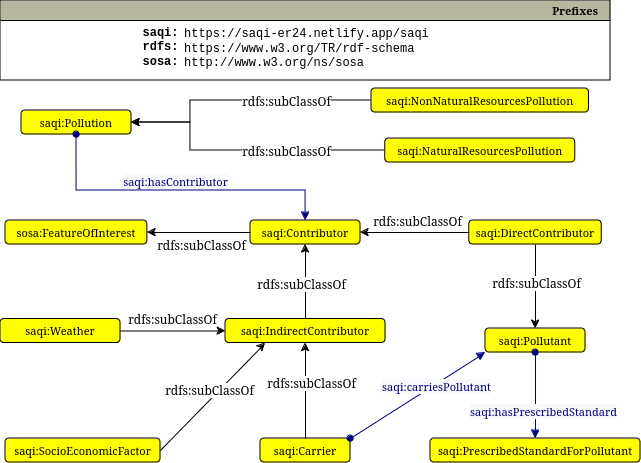
\includegraphics[height=6.8cm]{figures/ODP_subset_new.png}
\caption{Main concepts and properties of the Pollution module} 
\label{fig:pollution-module}
\end{figure}

%The sensors, observations, samples and actuator (SOSA) ontology includes concepts related to sensors and their observations. We derived \texttt{Contributor} from \href{http://www.w3.org/ns/sosa/FeatureOfInterest}{sosa:FeatureOfInterest}. With this, we can describe sensor observations with time and spatial information. The \href{https://www.w3.org/2003/01/geo/wgs84_pos#}{WGS84} vocabulary provides \href{http://www.w3.org/2003/01/geo/wgs84_pos#SpatialThing}{SpatialThing} for describing a spatial location on Earth. Figures~\ref{fig:reused-concepts-wgs84-sosa}, \ref{fig:air_pollution_concepts}, and \ref{fig:contributor_concepts} capture these re-used concepts in SAQI ontology. %We have also resused \href{http://xmlns.com/foaf/0.1/#term_Agent}{foaf:Agent} and schema TODO - ODPS, shcema, foaf etc.
 
\begin{figure}[ht]
\centering
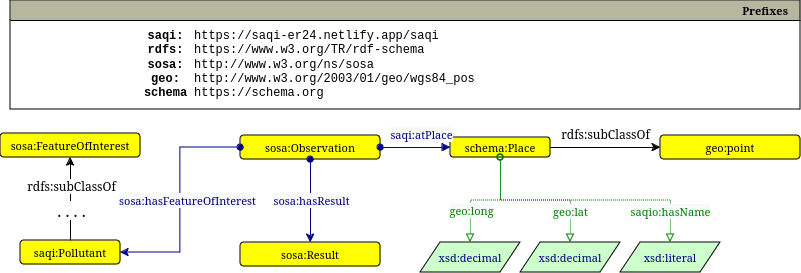
\includegraphics[height=3cm]{figures/reuse_new.png}
\caption{Re-used concepts from WGS84 and SOSA} 
\label{fig:reused-concepts-wgs84-sosa}
\end{figure}


\textbf{AirPollution.} This class is extended from the \texttt{Pollution} class of the Pollution ODP. The \texttt{Pollution} class represents the different types of contaminants in the natural environment. \texttt{AirPollution} is linked to \texttt{Pollutant} through the  \texttt{hasContributor} property (Axiom 1). The institutions working to mitigate the pollution sources through policies and awareness campaigns are linked by the object property \texttt{takesActionAgainst}. These properties and their connection with the \texttt{AirPollution} class are shown in Figure~\ref{fig:air_pollution_concepts}.

\begin{equation}
    \texttt{Pollution} \sqsubseteq \exists\texttt{hasContributor}.\texttt{Contributor}    
\end{equation}

\begin{figure}[ht]
\centering
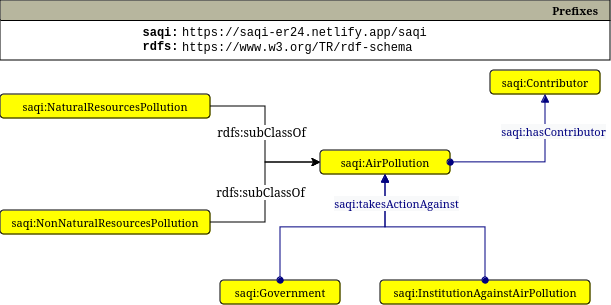
\includegraphics[height=4.5cm]{figures/airpoll_new.png}
\caption{AirPollution class and its connections} 
\label{fig:air_pollution_concepts}
\end{figure}

\textbf{hasContributor.} This object property connects the \texttt{AirPollution} class to its direct and indirect contributors (pollutants). %represent Direct or Indirect contributors that cause a particular kind of Pollution. In SAQI context, only, all contributors are linked to AirPollution instance of pollution.

\textbf{takesActionAgainst.} The institutions that are working to mitigate the effects of air pollution are connected through this object property. We considered two possible types of institutions -- government and non-government institutions such as NGOs. %that actively work on either reducing the pollutants causing Pollution, or reduce exposure to pollution in their geographical area of focus.

\textbf{Contributor.} It is a subclass of \href{http://www.w3.org/ns/sosa/FeatureOfInterest}{sosa:FeatureOfInterest},  allowing us to record observations of the contributors. A contributor can either be a contaminant particle, i.e., \texttt{Pollutant} or it could be a \texttt{Carrier} that transports a \texttt{Pollutant}. The \texttt{Contributor} class and other related classes are shown in Figure~\ref{fig:contributor_concepts}.

\begin{figure}[ht]
\centering
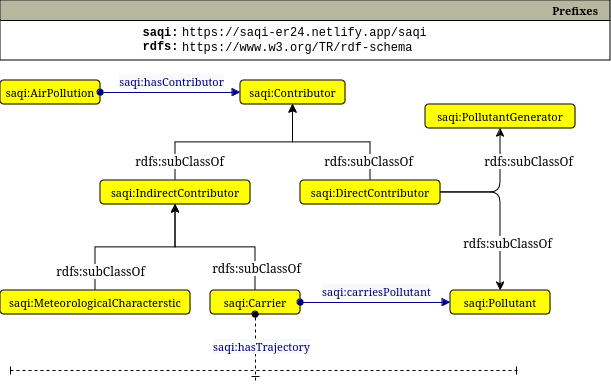
\includegraphics[height=6cm, width=0.80\textwidth]{figures/contrib_new.png}
\caption{Contributor class and its connections} 
\label{fig:contributor_concepts}
\end{figure}

\textbf{carriesPollutant.} This object property is used with an  \texttt{IndirectContributor} that transports a \texttt{Pollutant} from one spatial location to another, for example, wind and water flow.

\textbf{DirectContributor.} This class represents the contributors that directly impact pollution. \texttt{Pollutant} is a subclass of \texttt{Direct\-Contributor}. Some examples of pollutants include biological pollutants (viruses, pathogens, bacteria, etc.), chemical pollutants (toxic metal, radionuclides, organophosphorus compounds, gases, etc.) and physical pollutants (sound, thermal energy, space debris, etc.) present in the environment. 

\textbf{IndirectContributor.} This represents the things that indirectly contribute to pollution at a particular spatiotemporal point. These include environmental factors like temperature, the air or water streams flowing into or out of a particular place, the socio-economic factors such as policies and demographics. We have modelled only the \texttt{Carrier} concept as the subclass of \texttt{IndirectContributor} since other indirect contributors are specific to certain kinds of pollution.

\textbf{Carrier.} This concept is a subclass of the \texttt{IndirectContributor} concept and represents the air, water, and other kinds of streams flowing into or out of a particular place. It is linked to the \texttt{Trajectory} concept through the \texttt{hasTrajectory} property. Carriers are generally observed to affect the concentration of pollutants at a particular place and are important in modelling pollutants. To represent the pollutants that might be carried through a trajectory, the \texttt{Carrier} concept is linked to the \texttt{Pollutant} concept by the \texttt{carriesPollutant} property. %To specify the location of the source of pollutants in a carrier trajectory, \texttt{nearby} property can be used. This links the pollutant sources such as factories in the case of wind stream carrier or drains in the case of water stream carrier to the \texttt{TrajectoryPoint}. The applications that have such a requirement can make use of the \texttt{nearby} property, but we excluded it from the ODP because it is not sufficiently general.


\textbf{Pollutant.} \texttt{Pollutant} is a central concept in the Pollution module. It is  associated with the \texttt{Observation} class to keep a record of pollutant concentrations at any location and timestamp. Each pollutant has a prescribed standard that is defined by the government authorities. The \texttt{Pollutant} class and its connections are shown in Figure~\ref{fig:pollutant_concepts}. %The carrier concept can be used to track the flow of pollutants through location and time.

%\textbf{carriesPollutant.} Links an \texttt{IndirectContributor} which transports a \texttt{Pollutant} from one spatial location to another, for example, wind and water flow.

\textbf{hasPrescribedStandard.} Links a pollutant with standard limits based on concentration/amount of that pollutant in the environment. For example, WHO prescribed standard for PM$_{2.5}$ is less than 5 $\mu g/m^3$ mean concentration in the air annually. 

\textbf{hasObservation.} This is used to capture the concentration of a particular pollutant at a given time and spatial location.
    %\footnote{2005 WHO guidelines prescribe the  range for air pollutants such as particulate matter (PM), ozone ($O_3$), nitrogen dioxide ($NO_2$), etc., available at  \href{http://whqlibdoc.who.int/hq/2006/WHO\_SDE\_PHE\_OEH\_06.02\_eng.pdf}{http://whqlibdoc.who.int/hq/2006/WHO\_SDE\_PHE\_OEH\_06.02\_eng.pdf}}

\begin{figure}[ht]
\centering
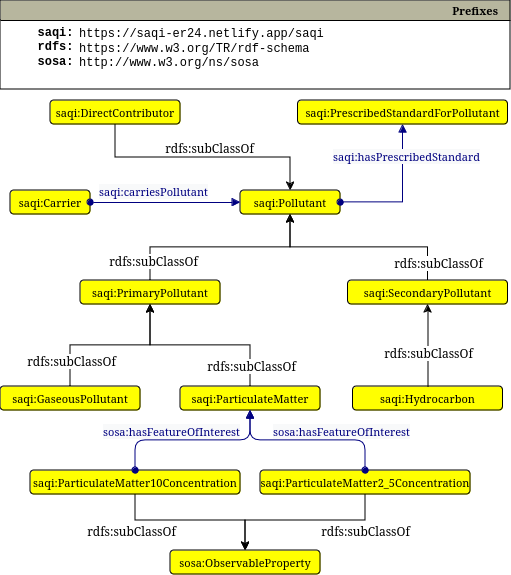
\includegraphics[height=8cm]{figures/pollutants_new.png}
\caption{Pollutant class and its connections} 
\label{fig:pollutant_concepts}
\end{figure}
    
\textbf{PrescribedStandardForPollutants.} This is a stub meta-pattern~\cite{stub_MP} that can be used to describe the prescribed ranges for pollutants. For a particular location, pollutants have a defined range of permissible concentrations that are specified by various global authorities. A standard for a pollutant may change with time and place. Hence the \texttt{PrescribedStandardFor\-Pollutant} concept is linked to the \texttt{Observation} concept by the \texttt{has\-Observation} property.

\textbf{PollutantGenerator.} Pollutant generators are events that generate pollution, such as crop burning, power plants, waste burning and dusty weather. It is related to the \texttt{Perception} class in the \emph{Ethnography} module, indicating the  perception of people on the severity of pollution concentration in a specific area. The \texttt{PollutantGenerator} class and its connections are shown in Figure~\ref{fig:pollutant_generator}.

\textbf{nearby.} This property links a pollution generator to a carrier trajectory.

\textbf{sourceResponsibleForLocalPollution.} The perception of pollution is directly linked to observable pollution generators in a locality, resulting in the perception of pollution by the people in that locality.


\begin{figure}[ht]
\centering
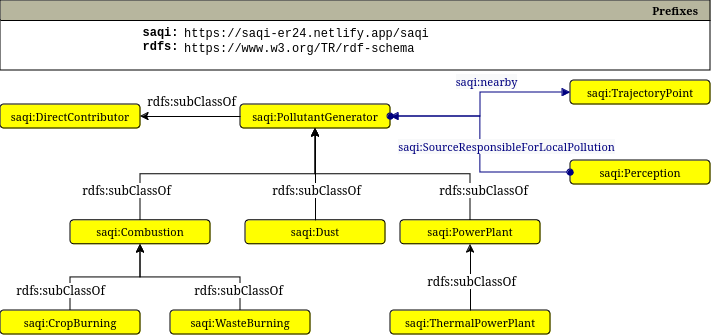
\includegraphics[height=6cm]{figures/pollutant_generator_new.png}
\caption{PollutantGenerator class and its connections} 
\label{fig:pollutant_generator}
\end{figure}


\subsection{Trajectory Ontology}

Concepts in the \emph{Trajectory} module use the concepts from the Pollution ODP (Figure~\ref{fig:trajectory_concepts}). It models the trajectories of pollution carriers. For example, a wind current passing through a crop burning site may carry carbon based pollutants to another destination. This displacement of pollutants needs to be accounted for to get a holistic understanding of air pollution. The trajectory component has been adapted from the Trajectory ODP~\cite{10.1007/978-3-319-01790-7_24}. A brief description of the \emph{Trajectory} module concepts is as follows.

\begin{figure}[ht]
\centering
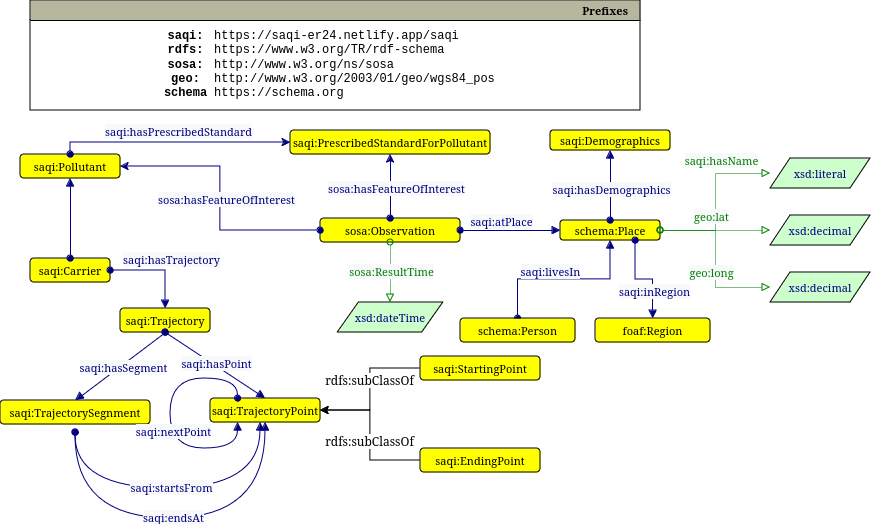
\includegraphics[height=6.5cm, width=0.90\textwidth]{figures/ObservationTrajectory.png}
\caption{Trajectory class and its connections} 
\label{fig:trajectory_concepts}
\end{figure}

\textbf{Trajectory.} The \texttt{Trajectory} concept represents a set of ordered spatiotemporal points. 

\textbf{TrajectoryPoint and TrajectorySegment.} The \texttt{Trajectory} concept is linked to the \texttt{TrajectoryPoint} and \texttt{TrajectorySegment} through the \texttt{hasPoint} and \texttt{hasSegment} properties. The \texttt{nextPoint} property links trajectory points in the
appropriate order within a trajectory. The segments in the trajectory are defined by a starting trajectory point \{$x_i$, $y_i$, $t_i$\} and an ending trajectory point \{$x_j$, $y_j$, $t_j$\} where $t_i$, $t_j$ denote time points such that $t_i$ $<$ $t_j$ . The \texttt{TrajectorySegment} concept represents this notion of a segment which is connected to two fixes through \texttt{startsFrom} and \texttt{endsAt} properties.

%\begin{figure}[ht]
%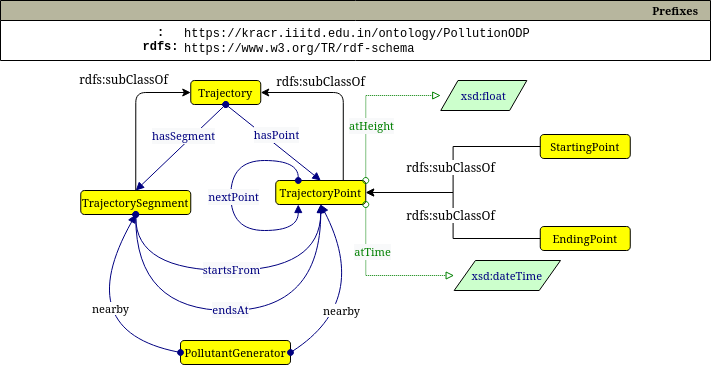
\includegraphics[ height=4.5cm]{figures/Trajectory.png}
%\caption{Trajectory concepts in PollutionODP} 
%\label{fig1}
%\end{figure}
\subsection{Ethnography Ontology}
This ontology captures the ethnographic details of a location we obtained from the field survey. This data and the ontology can help frame policies and make decisions to mitigate air pollution at the hyperlocal level. The \emph{Ethnography} module is shown in Figure~\ref{fig:ethnographic_concepts}.

\begin{figure}[ht]
\centering
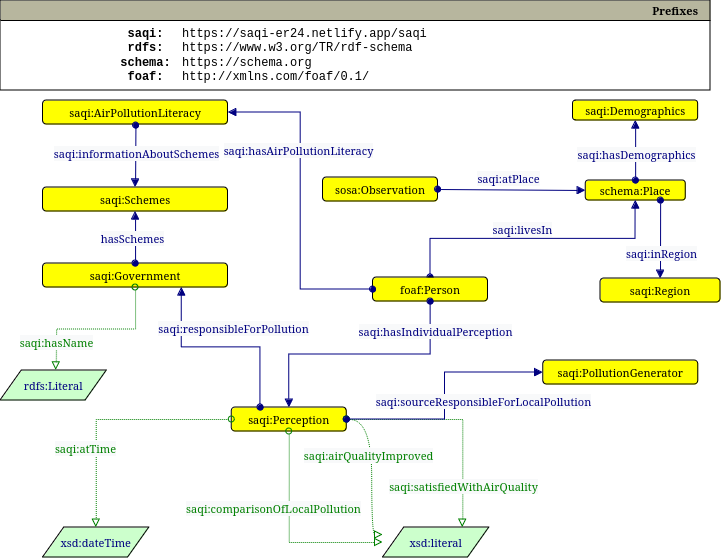
\includegraphics[height=6.5cm]{figures/Ethnography.png}
\caption{Overview of the Ethnography module} 
\label{fig:ethnographic_concepts}
\end{figure}

\textbf{Person.} This is a core concept of this module since the ethnographic data relies on the observations of a person. The data we collect relates a person to their knowledge of air pollution and accounts for the social makeup through the aggregation of person-level data. This concept is connected to concepts such as \texttt{AirPollutionLiteracy}, \texttt{Perception} and \texttt{Region} through the \texttt{hasAirPollution\-Literacy}, \texttt{hasPerception} and \texttt{livesIn} properties.

\textbf{AirPollutionLiteracy.} This concept describes the air pollution literacy of the people in a locality. We assess this by asking questions\footnote{The questionnaire for collecting ethnographic data has been designed by social scientists in our team.} to the people related to their awareness of AQI and air pollution in general. The \texttt{AirPollutionLiteracy} concept has the data properties \texttt{hasAQILiteracy}, \texttt{hasAirPollutionGraphic\-Literacy}, \texttt{hasParticulateMatterLiteracy} and \texttt{hasAQIColorLiteracy}. 

\textbf{Perception.} This concept captures the perception of an individual with regard to the level of air pollution in their local neighbourhood and the city. It consists of data properties such as \texttt{howIsYourLocalityComparedToOtherAreas} (the literals that can be linked using this property are ``equally polluted'', ``less polluted'', ``more polluted'', ``don't know''), \texttt{shouldPollutionIssuesBeRaisedIn\-Elections} and \texttt{localAirQualityRating}. An aggregation of people's perceptions in a particular region is expected to give the perception of that region.


\section{SHACL Shapes}
\label{sec:shacl}

SHACL\footnote{\url{https://www.w3.org/TR/shacl/}} can be used to enforce constraints on the KG. The constraints are defined in shape graphs. KG must satisfy the condition specified in the shape graphs to be validated. Shapes for the classes were created, and the triples generated from the data using YARRRML mappings were validated using the SHACL constraints. A snippet of the SHACL shape for the \texttt{Person} class is given in Listing~\ref{shacl-person}. It describes the constraint that a person can wear exactly one mask. The rest of the SHACL constraints are available at \url{https://github.com/kracr/aq-structured-platform/tree/main/dataset/SHACL-shapes}. %The first few constraints indicate that the subject (\texttt{Person} in this case) should have one and exactly one value associated with a property (for example, \texttt{saqi:livesIn}).

\begin{lstlisting}[label=shacl-person,caption=SHACL constraints snippet for the Person class,float,frame=tb,captionpos=b]
    sh:property [
      rdf:type sh:PropertyShape ;
      sh:path saqi:wearsMask ;
      sh:datatype xsd:boolean ;
      sh:maxCount 1 ;
      sh:minCount 1 ;
      sh:name "wears mask" ;
    ] ;

    sh:targetClass saqi:Person ;
    sh:targetSubjectsOf saqi:hasAirPollutionLiteracy ;
    sh:targetSubjectsOf saqi:hasIndividualPerception ;
    sh:targetSubjectsOf saqi:livesIn ;
\end{lstlisting}

%\begin{verbatim}
%    saqi:PersonShape
%  rdf:type sh:NodeShape ;
%  sh:property [
%      rdf:type sh:PropertyShape ;
%      sh:path saqi:hasAirPollutionLiteracy ;
%      sh:class saqi:Person ;
%      sh:maxCount 1 ;
%      sh:minCount 1 ;
%      sh:name "has air pollution literacy" ;
%      sh:nodeKind sh:IRI ;
%    ] ;
%  sh:property [
%      rdf:type sh:PropertyShape ;
%      sh:path saqi:hasPerception ;
%      sh:class saqi:Person ;
%      sh:maxCount 1 ;
%      sh:minCount 1 ;
%      sh:name "has individual perception" ;
%      sh:nodeKind sh:IRI ;
%    ] ;
%  sh:property [
%      rdf:type sh:PropertyShape ;
%      sh:path saqi:livesIn ;
%      sh:class saqi:Person ;
%      sh:description "Person lives in a particual region" ;
%      sh:maxCount 1 ;
%      sh:minCount 1 ;
%      sh:name "lives in" ;
%      sh:node saqi:PersonShape ;
%      sh:nodeKind sh:IRI ;
%    ] ;
%  sh:property [
%      rdf:type sh:PropertyShape ;
%      sh:path saqi:usesAirPurifier ;
%      sh:datatype xsd:boolean ;
%      sh:maxCount 1 ;
%      sh:minCount 1 ;
%      sh:name "uses air purifier" ;
%    ] ;
%  sh:property [
%      rdf:type sh:PropertyShape ;
%      sh:path saqi:wearsMask ;
%      sh:datatype xsd:boolean ;
%      sh:maxCount 1 ;
%      sh:minCount 1 ;
%      sh:name "wears mask" ;
%    ] ;
%  sh:targetClass saqi:Person ;
%  sh:targetSubjectsOf saqi:hasAirPollutionLiteracy ;
%  sh:targetSubjectsOf saqi:hasIndividualPerception ;
%  sh:targetSubjectsOf saqi:livesIn ;
%.
%saqi:actsThrough
%  rdf:type sh:PropertyShape ;
%.
%saqi:hasAirPollutionLiteracy
%  rdf:type rdf:Property ;
%.
%saqi:hasPerception
%  rdf:type rdf:Property ;
%.
%saqi:livesIn
%  rdf:type rdf:Property ;
%.
%\end{verbatim}

\section{SAQI Application}
\label{sec:app}
We built a mobile and Web friendly SAQI application (Figure~\ref{fig:saqi_layout})\footnote{Web version of the app can be accessed live at \url{https://w3id.org/saqi/app}.} that makes use of the KG to answer questions related to air quality.\footnote{The uploaded data in KG consists of ~3.4 million triples mostly from sensors data collected over 4 months} To mitigate the knowledge barrier in understanding AQI, increase awareness related to air pollution and improve citizen engagement, the app is designed to address all the sections of the community, including the tech ill-literate people. This is achieved using features such as support for local language -- Hindi/English, heavy/large fonts, minimal user input, text-to-speech narration on every page and colourful graphics for AQI readings. The app consists of knowledge on air pollution and its effects which caters to specific social and spatial cohorts and also acts as AQI monitoring app that utilizes a KG built using SAQI ontology. 

\begin{figure}[ht]
\centering
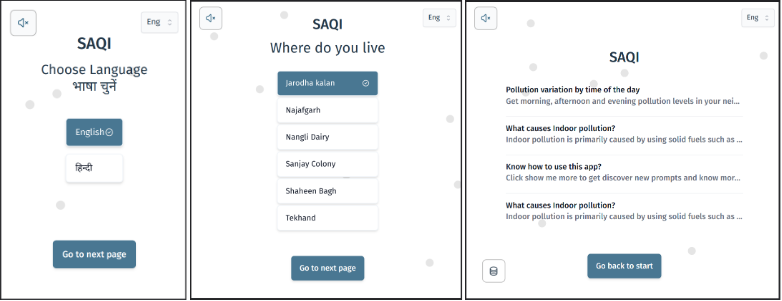
\includegraphics[ height=4.5cm]{figures/saqi_app_layout.png}
\caption{User interface of the SAQI app. Each screen has only one clickable input with large, clear fonts with minimal content} 
\label{fig:saqi_layout}
\end{figure}

A SPARQL endpoint (Figure~\ref{fig:saqi_sparql}) is also embedded in the application with eight queries on the pollution sensors data and the ethnography data from surveys. The SPARQL endpoint can be accessed from the app at  \url{https://w3id.org/saqi/app/#/sparql}. The ethnographic data, pollution data from local and central sensors are mapped to triples using RDF Mapping Language (RML) helper tool YARRML\footnote{\url{https://rml.io/yarrrml/}.}~\cite{YARRRML} that provides a high level format to define R2RML and RML rules. The generated triples are loaded into a server running Apache Jena Fuseki\footnote{\url{https://jena.apache.org/documentation/fuseki2/}.} as the triple store. A cron job running on the server updates the KG with the new triples and validates the KG using SHACL constraints.

 \begin{lstlisting}[label=lst:saqi-query,caption={An example of a SPARQL query used by saqi; output of this query is present in Table~\protect\ref{saqi-query-result}},float,frame=tb,captionpos=b,basicstyle=\ttfamily\small]
 
# The query returns average pollutants in specific time bands
  PREFIX rdf: <http://www.w3.org/1999/02/22-rdf-syntax-ns#>
  PREFIX rdfs: <http://www.w3.org/2000/01/rdf-schema#>
  PREFIX saqi: <https://kracr.iiitd.edu.in/ontology/saqi#>
  PREFIX xsd: <http://www.w3.org/2001/XMLSchema#>
  PREFIX sosa: <http://www.w3.org/ns/sosa/>
  
  SELECT (AVG(?pm10Instance) AS ?pm_10) 
  (AVG(?pm25Instance) AS ?pm_25) ?timesofday WHERE {
    ?obs_pm_25 a sosa:Observation .
    ?obs_pm_25 sosa:resultTime ?time .
    ?obs_pm_25 saqi:atPlace ?place .
    ?obs_pm_25 saqi:madeBySensor ?source .
    ?obs_pm_10 a sosa:Observation .
    ?obs_pm_10 sosa:resultTime ?time .
    ?obs_pm_10 saqi:atPlace ?place .
    ?obs_pm_10 saqi:madeBySensor ?source .
  	# Add location name or time interval filter
    FILTER (
      ?time > "2021-11-01T00:00:00+05:30"^^xsd:dateTime &&
      ?time < "2021-11-10T00:00:00+05:30"^^xsd:dateTime
    )
    ?obs_pm_25 sosa:observedProperty saqi:ParticulateMatter2_5Concentration .
    ?obs_pm_25 sosa:hasResult ?pm25Instance .
    ?obs_pm_10 sosa:observedProperty saqi:ParticulateMatter10Concentration .
    ?obs_pm_10 sosa:hasResult ?pm10Instance .
  	?place saqi:hasName ?placeName .
	  ?source rdfs:label ?dataSource .
    BIND (hours(?time) AS ?hour)
    OPTIONAL { FILTER (?hour <= 8)
      BIND("Morning" AS ?timesofday)
    }
    OPTIONAL { FILTER (?hour > 8 && ?hour <= 16)
      BIND("Afternoon" AS ?timesofday)
    }
    OPTIONAL { FILTER (?hour > 16 && ?hour <= 20)
      BIND("Evening" AS ?timesofday)
    }
    OPTIONAL { FILTER (?hour > 20)
      BIND("Night" AS ?timesofday)
    }
  } 
  GROUP BY ?timesofday
  LIMIT 10000
\end{lstlisting}

\begin{table}[!h]
\begin{center}
\caption{Result of SPARQL Query from Listing~\ref{lst:saqi-query}}
\label{saqi-query-result}
\begin{tabular}{|c c c|} 
 \hline
 pm\_10 & pm\_25 & timesofday \\ [0.5ex] 
 \hline\hline
 331.96637 & 282.92276 & Morning \\ 
 \hline
 381.802 & 332.8371 & Night \\
 \hline
 302.69052 & 260.283 & Afternoon \\
 \hline
 335.77588 & 285.6778 & Evening \\ [1ex] 
 \hline
\end{tabular}
\end{center}
\end{table}

 %\footnote{Apache Jena Fuseki \url{https://jena.apache.org/documentation/fuseki2/}.}
 
\begin{figure}[ht]
\centering
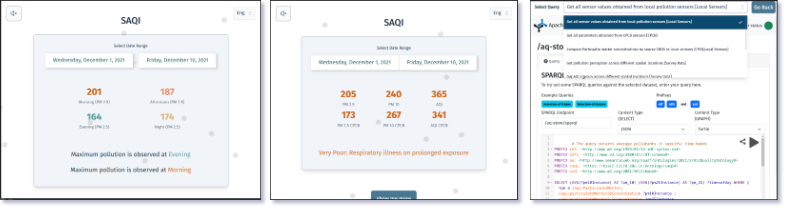
\includegraphics[ height=3.5cm]{figures/saqi_sparql.png}
\caption{Screenshots of the app using SPARQL queries to answer questions. The SPARQL endpoint screen is also shown here.} 
\label{fig:saqi_sparql}
\end{figure}

%\subsection{Methodology}

\subsection{Evaluation}
To evaluate the SAQI app, we conducted a user survey across the six locations where the local sensors were deployed. There were 60 participants spread across each of the six social cohorts. There were an equal number of male and female participants, and the age range of the participants was between 17 and 57 years. The questions to the participants were on media and digital literacy, AQI and air pollution awareness, the app's usability and utility, and community building after using the app. We used the Likert scale (1 to 5) for several questions, with 1 depicting the best case scenario and 5 the worst case. The feedback on the app was largely positive. The app got a usability score of $\sim$1.8, and a utility score of $\sim$2.1 on the understanding of AQI and $\sim$2.25 on suggestions to handle air quality in a local region. This is shown in Figure~\ref{fig:evaluation}. The survey also captures feedback on the improvements to the app, which is available after anonymization at \url{https://doi.org/10.5281/zenodo.10300235}. 

\begin{figure}
    \centering
    \begin{subfigure}[b]{0.38\textwidth}
        \centering
        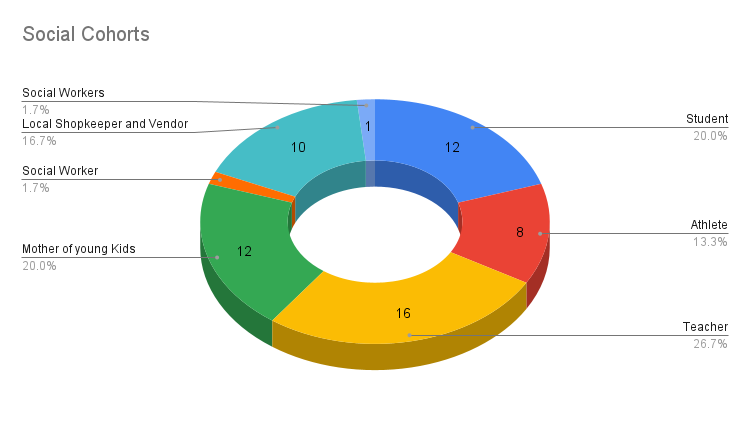
\includegraphics[width=\textwidth]{figures/evaluation2.png}
        \caption{Demographics}
        \label{fig:demographics_evaluation}
    \end{subfigure}
    \hfill
    \begin{subfigure}[b]{0.6\textwidth}
         \centering
         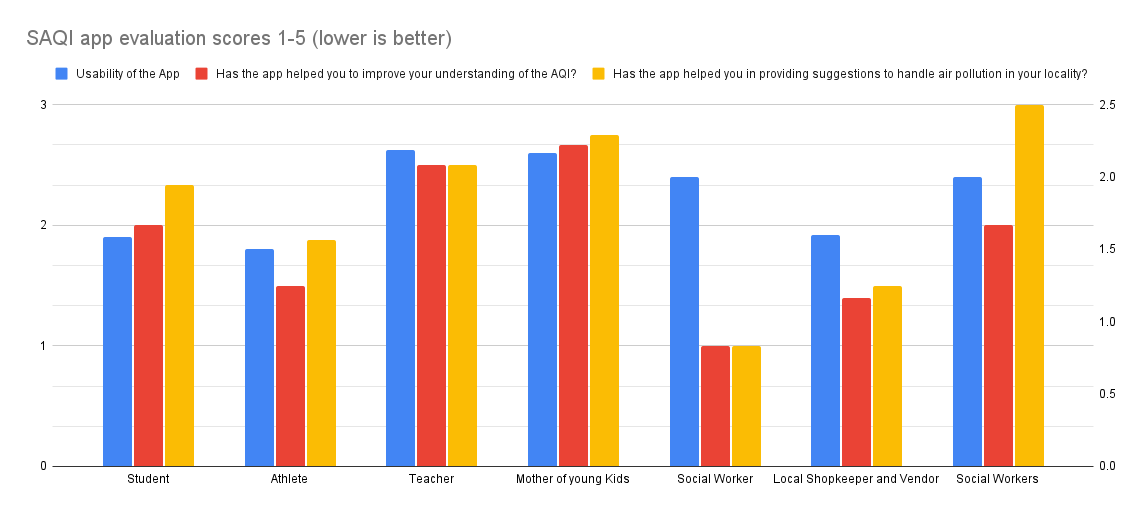
\includegraphics[width=\textwidth]{figures/evaluation.png}
         \caption{Evaluation scores}
         \label{fig:scores_evaluation}
     \end{subfigure}
    \caption{SAQI App evaluation results}
    \label{fig:evaluation}
\end{figure}

% \begin{figure}[ht]
% \centering

% 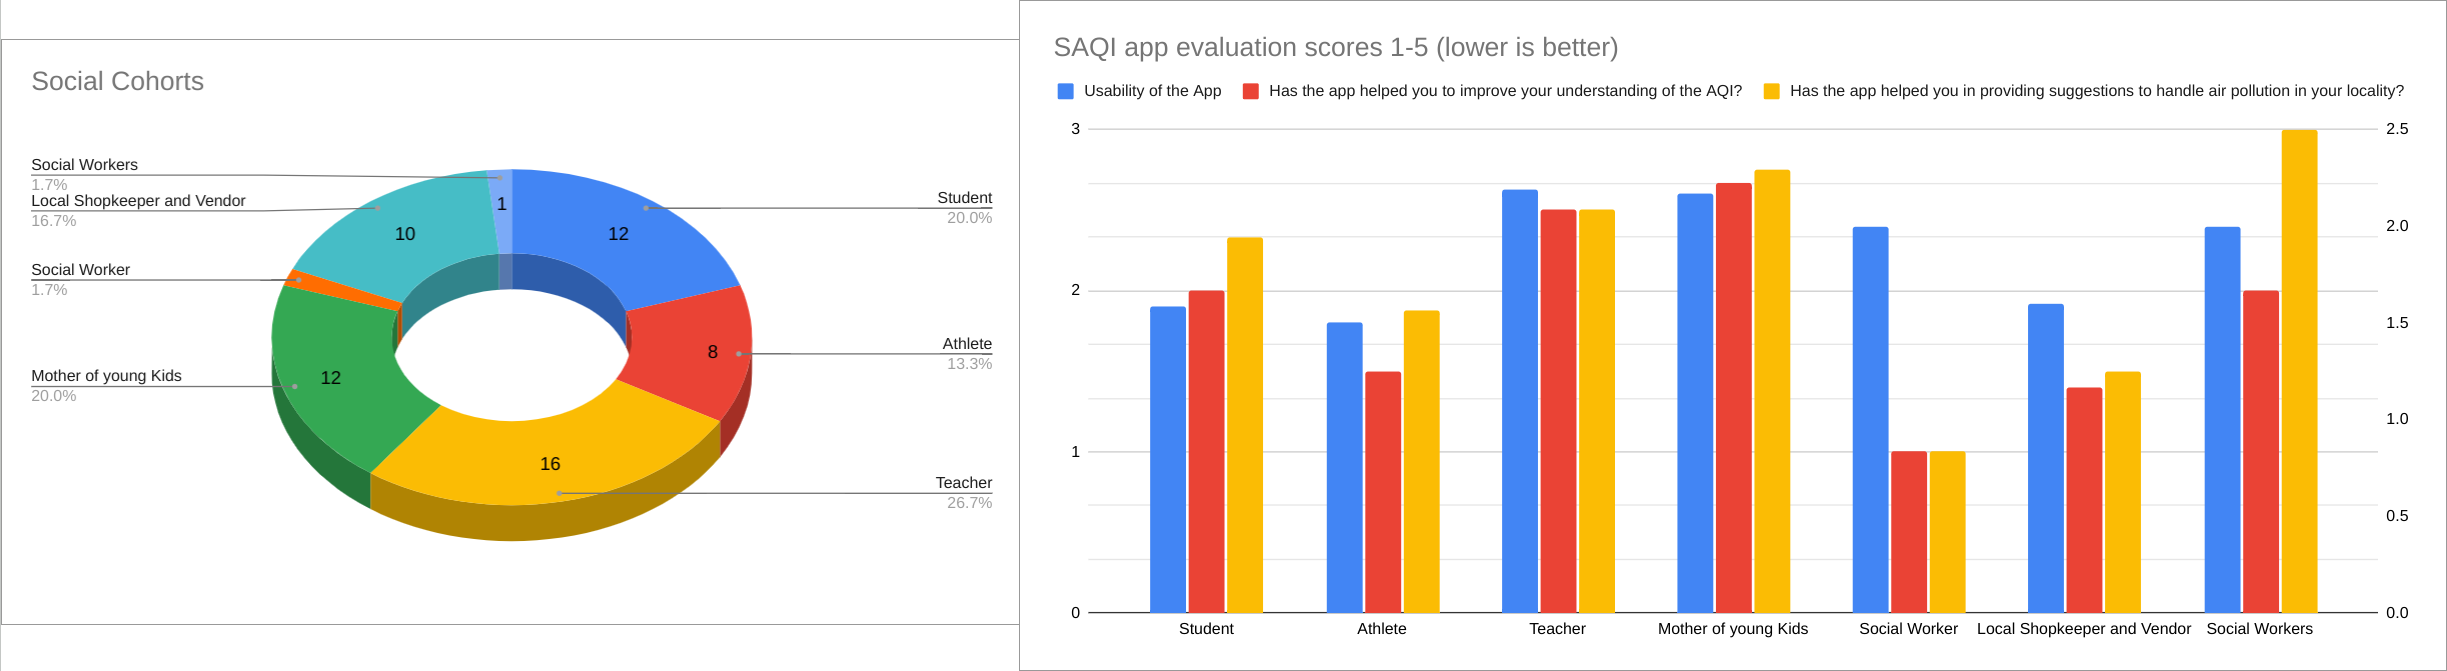
\includegraphics[height=3.5cm]{figures/saqiapp.png}
% \caption{Evaluation demographics and score for saqi app} 
% \label{fig:saqi_evaluation}

% \end{figure}

% TODO - add survey result summary, describe demographics - results - average rating questions(imp ones - usability, use fullness), summarize others. Add diagram - 3 graphs in one fig call them a,b,c.(like pie chart). Add some discussion points on them.
% Approx - 2 paras.

% DROP election
\section{Sustainability and Maintenance of Resources}
\label{sec:sustainability}

Since the YARRRML mappings are used, it is easy to generate KG from air quality sensor data and survey data. This is scalable, i.e., we can expand to more regions and get more data. As long as the format of the data does not change, the process of converting heterogeneous sensor and survey data to KG is sustainable. Over time, the SAQI ontology and the application may need changes. We will continue to work on SAQI platform and make changes whenever required. We also hope that the community will be interested and will take this up. Since all the resources are publicly available, it is possible to make changes and share them with the community. 

%KRACR lab \footnote{Kracr lab - \url{https://kracr.iiitd.edu.in}} is hosting the SAQI knowledge graph and the live version of app through infrastructure provided by IIIT Delhi. The data is available as triples through the server hosted at \url{https://kracr.iiitd.edu.in/sparql} and the raw data files along with mapping scripts, and processed csv files are hosted through zenodo \footnote{Zenodo - \url{https://zenodo.org/}}.
\section{Conclusion and Future Work}
\label{sec:conclusion}

We proposed Social Air Quality Index (SAQI), a new approach to increase awareness about air pollution,  democratize AQI knowledge at the neighbourhood level and improve community participation. We developed a SAQI ontology to model the local and central air quality data and the ethnographic survey data from six localities in Delhi. The sensor and survey data are integrated into a KG using YARRRML mappings. We designed a neighbourhood pollution dashboard (SAQI app) that uses the KG to answer questions related to air pollution and the steps that each social cohort (students, teachers, mothers of young kids, athletes, etc.) can take to mitigate the effects of air pollution. The app has received positive feedback on its usability and utility. All these resources are publicly available under an Apache License 2.0 at \url{https://github.com/anon-DC1E/SAQI-ER-24} and \url{https://doi.org/XX.XXXXX/zenodo.XXXXXXXX}. 

In the future, we plan to incorporate more social characteristics from the neighbourhood into the ontology and the SAQI app, such as addresses and contacts for local government officials and the local pollution generating sources. We also plan to introduce graphical visualization in the app to explain the distribution and variation of AQI with respect to the time of the day, the seasonal variations and its correlation to activities in the neighbourhood.

%\textbf{Acknowledgement.} The ***** ***** for ******** ************ (CAI), *****-*****, India has partially supported this work.

\bibliographystyle{splncs04}
\bibliography{bibliography}

\end{document}
